%
\hsection{Relationships}%
\label{sec:conceptual:relationships}%
%
If we only had a single entity type in our \db, the using a \db\ makes no sense.
In that case, we would be better of using simple documents, like \pgls{CSV} or \pgls{XML} files.
However, clearly, in our teaching management platform application, we are going to have many different entity types.
And again, if these entity types were unrelated, say \inQuotes{Student,} \inQuotes{Weather,} \inQuotes{Product,} then we were still better off storing them in a bunch of such files.
But they are related.
So how do we model these relationships?
Let us begin with some basic definitions~\cite{G2011EW2ITDS:CMUTERM}.%
%
\begin{definition}[Relationship]%
A \emph{relationship}~(instance) is an association of two or more entities.%
\end{definition}%
%
An example for a relationship would be \emph{Mr.~Bibbo enrolls into the module \citetitle{programmingWithPython}.}
%
\begin{definition}[Relationship Type]%
A \emph{relationship type} is the set of all relationships possible between two or more sets of entities.%
\end{definition}%
%
The \emph{Enrolls} relationship type could be defined between the \emph{Student} entity type and the \emph{Module} entity type.
We notice that~(transitive) verbs~\cite{EOWM2025MWAMTD:TA} in the requirements definition often represent relationship types~\cite{C1997ECAED}.%
%
\begin{definition}[Degree of Relationship]%
\label{def:degreeOfRelationship}%
The degree of a relationship~(instance or type) refers to the number of participating entities.%
\end{definition}%
%
There can be binary relationships, i.e., relationships where two entities participate.
For example, we could model the student-module relationship in a binary fashion: \emph{Student enrolls into Module.}
We could just as well use a ternary relationship with three participating entities instead, e.g., \emph{Student enrolls into Module taught by Professor.}
%
\begin{definition}[Roles in a Relationship]%
Each entity participating in relationship may have a role, which defines the way in which the entity participates in the relationship.%
\end{definition}%
%
If we imagine the ternary \emph{Student enrolls into Module taught by Professor} relationship, then the student could have the role \emph{enrolls} and the professor could have the role \emph{teaches}.%
%
\begin{definition}[Relationship Attribute]%
\label{def:relationshipAttribute}%
A relationship type can have attributes describing properties of the relationship.%
\end{definition}%
%
For example, we could write something like \emph{Mr.~Bebbo enrolls into module \citetitle{databases} in summer semester 2025.}
The attribute \emph{Semester} of this relation only makes sense in this context.
It neither belongs to the student \emph{Mr.~Bebbo} nor does it belong to the module~\citetitle{databases}.
Different from entities, relationship types do not have key attributes.
The single relationships are identified by the primary keys of the participating entities~\cite{G2011EW2ITDS:CMUTERM}.

\begin{figure}%
\centering%
%
\subfloat[][%
The binary relationship of student and modules, which does not represent the relationship of professors to modules and students.%
\label{fig:erdStudentModule1}%
]{\parbox{0.99\linewidth}{\centering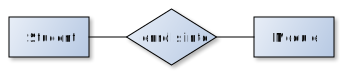
\includegraphics[scale=0.6]{\currentDir/erdStudentModule1}}}%
%
\floatRowSep%
%
\subfloat[][%
Two binary relationships, i.e., the relationship of student to modules and the relationship of professors to modules. %
This does not represent that a student enrolls into a course taught by a professor. %
\label{fig:erdStudentModuleProf1}%
]{\parbox{0.99\linewidth}{\centering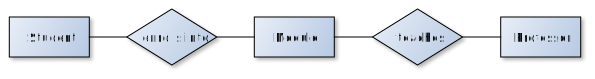
\includegraphics[scale=0.6]{\currentDir/erdStudentModuleProf1}}}%
%
\floatRowSep%
%
\subfloat[][%
The ternary relationship of students, modules, and professors. %
This represents how students join a course taught by a specific professor. %
However, it would not permit the same student enroll into the same course for two years. %
It also does not give us the information when the course takes place.%
\label{fig:erdStudentModuleProf2}%
]{\parbox{0.99\linewidth}{\centering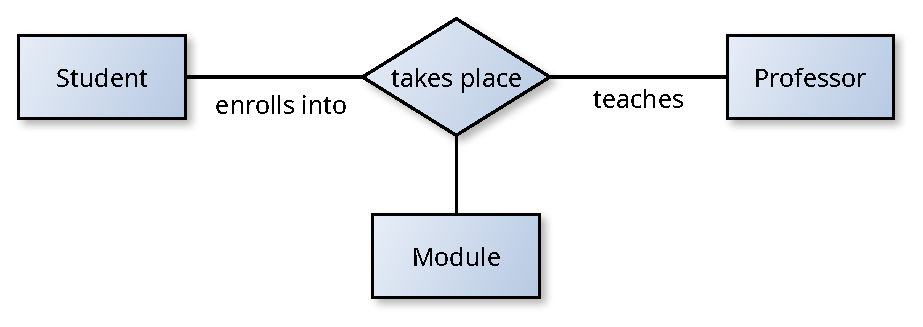
\includegraphics[scale=0.6]{\currentDir/erdStudentModuleProf2}}}%
%
\floatRowSep%
%
\xdef\erdStudentModuleProfIII{\currentDir/erdStudentModuleProf3}%
\subfloat[][%
The ternary relationship of students, modules, and professors with the relationship attribute semester.%
\label{fig:erdStudentModuleProf3}%
]{\parbox{0.99\linewidth}{\centering\includegraphics[scale=0.6]{\erdStudentModuleProfIII}}}%
%
\caption{Modeling the relationship between students, professors, and modules.}%
\label{fig:erdStudentModuleProf}%
%
\end{figure}%
%
Let us start modelling relationships.
We begin by representing the fact that a student can enroll into a module.
Relationships in \pglspl{ERD} are drawn as diamonds that are connected to the involved entities.
\Cref{fig:erdStudentModule1} shows an \pgls{ERD} where the student entity is linked to a module entity by the relationship \emph{enrolls into}.
This is a binary relationship, because two entities take part in it.

This diagram is interpreted as follows:
Entities of type student can enroll into an entities of type module.
At first glance, this sounds OK.
However, then we notice several problems with this.

First, modules are taught by professors.
This issue is not represented.
Matter of fact, the relationship makes no statement at all about this implicit student-professor relationship.

We try to fix this in \cref{fig:erdStudentModuleProf1} by adding a second binary relationship:
Professor teaches module.
Sadly, this does not solve the problem at all.
We now can properly represent that a student can enroll into a certain module.
We can also represent that a professor teaches a module.
But with this model, we cannot represent the information that a student joins a module taught be a specific professor.
Because the two binary relationships we drew are independent from each other.

This can be fixed by using a single ternary relationship in our model.
The \pgls{ERD} in \cref{fig:erdStudentModuleProf2} shows a relationship where three entity types participate.
The professor teaches the module and the student enrolls into the module that the professor teaches.
This model is much better.

However, it is still a bit ambiguous.
There is no real statement about when the module takes place.
Also, we said before that a relationship is represented by the primary keys of all involved entities.
What happens if a student takes part in a module but, sadly, fails the final exam or has to repeat the module for some other reason?
Can they enroll twice?
Well, if we use all the primary keys of all involved entities, i.e., one professor, one module, and potentially many students, that would probably be OK.
Although it feels awkward.
Also, what happens if the professor, for some reason, cannot complete the module and teaches it again next semester?
Then all the students would enroll again, and then we would definitely have two relations where all keys are identical.
To resolve these issues, we give our relationship the attribute \emph{in Semester} in \cref{fig:erdStudentModuleProf3}.

This was rather easy.
But let us do something a bit more interesting.
Today, we had a meeting with the stakeholders at the university again and showed them our entity model for students from \cref{fig:erdStudent5}.
It looks quite nice, we are told, but it does not withstand the harsh test of reality.

First, there is the issue with names again.
See, people may have \emph{multiple} names.
Foreign exchange students, for example, may have their original name.
However, they may \emph{also} have a Chinese name.
A Ms.~Elizabeth Prudence McDouglas may thus also be known as 邓小花 in the university.
Obviously, for official documents, only the original name of the person is to be used, while university-internal files or maybe seating cards in meetings might use the Chinesified name.
So the original name may be the name-for-documents, while others are there to allow us to match different documents.

\inQuotes{Original name,} we said, did we?
Actually, in the West, it is not uncommon that people change their name when they marry.
Let's say that Elizabeth marries Mr.~Heinrich Gieselher von G{\"o}rlitz-Zittau.
She may decide to keep her name unchanged.
She may take on the family name of her husband and become Mrs.~Elizabeth Prudence von G{\"o}rlitz-Zittau.
The couple may also choose for a composite family name.
This may result in a person named Mrs.~Elizabeth Prudence von G{\"o}rlitz-Zittau-McDouglas or maybe Mrs.~Elizabeth Prudence McDouglas-von-G{\"o}rlitz-Zittau.
(Notice that this would look interesting on Chinese official documents where the space for names is usually calculated to not exceed five characters\dots)
Either way, there can be a variety of reasons why names change.

However, changing the names in the \db\ is not an option.
Because this would mean that the old name \inQuotes{disappears}.
Then we would eventually have older documents in the real world that can no longer be matched with the updated data in the \db.
So we need to make names a multi-valued attribute, too.
When doing this, we may decide to assign names a valid-from and valid-from attribute, to emphasize the time when the names changed.

\begin{figure}%
\centering%
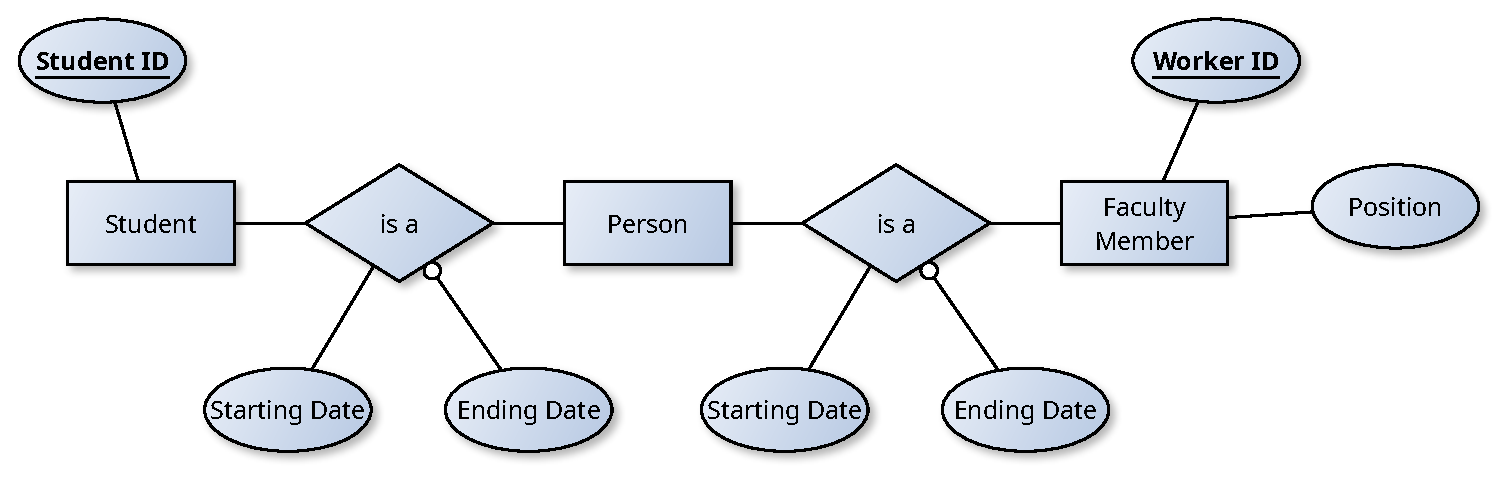
\includegraphics[scale=0.6]{\currentDir/erdPersonStudentFaculty1}%
\caption{An \pgls{ERD} illustrating the new \emph{Person} entity and how students and faculty members are related to it.}%
\label{fig:erdPersonStudentFaculty1}%
\end{figure}%

In the moment where wanted to begin modelling the names, we realize that this is not a student issue.
The same issue will later reappear when we model the employees of our university.
They, too, may have dodgy name issues.
They also have mobile phones, IDs, and addresses.
Now we do not want to model the same stuff twice, because that just makes the system more complicated and introduces the chance for inconsistencies.
Thus, before moving on, we decide to make short work of this problem by introducing a new entity \emph{Person}.
Students and employees are persons.
We will put all the fancy attributes then into the person records.
This also makes sense because, theoretically, a teacher might also enroll as a student.
Maybe a chemistry lecturer wants to also do a MSc in computer science.
Or a student first does the BSc in computer science and later the MSc.
They would still be the same person and there is no reason to store all their data separately multiple times.%

We sort out all of these issues in \cref{fig:erdPersonStudentFaculty1} by introducing the new entity type \emph{Person}.
Later, we will hang all the shared attributes on this entity type.
The entity type \emph{Student} for now only needs the single primary key attribute \emph{Student ID}.
A person can be a student and this relationship has a certain start and end date.
The end date can be \sqlilIdx{NULL} for all students that currently are enrolled and therefore is an optional attribute.

For faculty members, the situation is quite similar.
They are uniquely identified by a worker ID.
They also have a position, e.g., lecturer, associate professor, or full professor.
This function, too, has a start date and an optional end date.

\begin{figure}%
\centering%
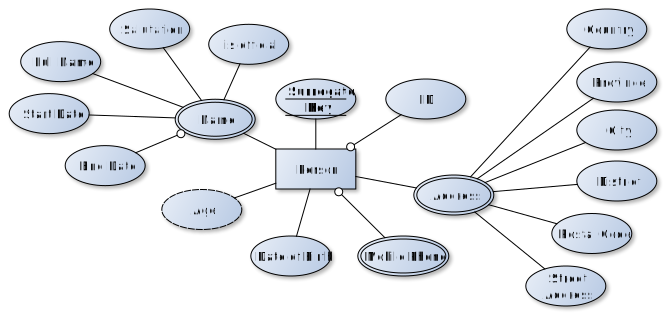
\includegraphics[scale=0.6]{\currentDir/erdPerson1}%
\caption{The \emph{Person} entity type with the attributes of the \emph{Student} entity type taken from \cref{fig:erdStudent5} and the improved \emph{Name} attribute.}%
\label{fig:erdPerson1}%
\end{figure}%
%
In \cref{fig:erdPerson1}, we copy the attributes from the \emph{Student} entity type in \cref{fig:erdStudent5} to the new \emph{Person} entity type.
Of course, we now do no longer include the student ID.
We also fix the \emph{Name} attribute.
It is now a multi-valued attribute.
Each name now also has a start and (optional) end date associated with it.
This should help to sort out situations such as name changes nicely.
We will also define the constraint that exactly one name of a person must be the \emph{offical} name and that this name must have a start date before the present date and no end date.

We imagine that our system will not bother the data-entry person too much with these options.
They can just enter one name.
Its start date will be set automatically to today and it will automatically be marke as official.
The system will automatically set the salutation and the full name to be the same.
The administrative person working with this data will be able to change either of them, to add new names, mark names as official, change dates, and so on.
So there would not be much hassle when entering the data but the \emph{option} to deal with all sorts of name-related issues.
And since our university is an international university with students and faculty from all over the globe, it is important to consider such issues from the beginning.

To our dismay, we realize one problem, though:
We can no longer spot a reasonable candidate for primary key in our \emph{Person} entity type.
\emph{Name} and \emph{Address} both are multi-valued composite attributes that do not need to be unique.
The government-issued \emph{ID} is optional.
The \emph{Mobile Phone} number is both optional and multi-valued.
\emph{Date of Birth} is certainly not unique and \emph{Age} is additionally derived.
None of them and neither combination is necessarily unique.
Of course, later, we will add other ID values like passport numbers and email addresses.
An application could enforce that each person has either a passport or a government-issued ID and that their numbers be unique.
However, it would still feel awkward to somehow create a Frankensteinesque primary key out of this.
The easiest solution here is to use a surrogate key.
In our model, we actually call it \emph{Surrogate Key,} to avoid any form of misunderstanding.
We will assume that whatever \dbms\ we will eventually use, it will be able to somehow generate unique values, like back in \dref{sec:factory:table:product}.
Our \emph{Person} in \cref{fig:erdPerson1} now looks fairly reasonable.

Having solved this problem, we now want to clean up the issue of IDs and ID documents.
So far, we modeled the ID as the government-issued ID.
It is an optional attribute, because foreign exchange students as well as foreign employees do not have one.
On one hand, even foreigners do have ID documents -- just not Chinese ones.
These are, of course, useless in our context.
On the other hand, a foreigner entering China must have a passport~\cite{ICAO2021MRTDP3SCTAMEE}.
A passport has a unique number {\dots} it is not a \emph{permanent} ID, though.
While Chinese~ID numbers stay the same, the passport number is usually a number identifying the passport booklet~\cite{ICAO2004TAGOMRTDFMUOPINAPN}.
A passport booklet usually stays valid for ten years and then a new passport is issued to the person, usually having a new passport number.
When a foreigner enters China, they need a visa, which, in turn, also has a unique identification number and a time window of duration~\cite{CMOFA2019ITCV}.
There are many different types of visa that have permit different activities, for example X1 and X2 for studying and Z~for working.
Foreigners who work in China~(e.g., as professors) furthermore need work permits~\cite{BD2006BDBK:WOFFITOROC}, which also have a unique numbers.
Of courses, visas and work permits eventually expire and need to be renewed.
This allows for an arbitrarily complex and ugly model.

\begin{figure}%
\centering%
\xdef\figErdPersonII{\currentDir/erdPerson2}%
\includegraphics[width=0.9999\linewidth]{\figErdPersonII}%
\caption{We now add the ID entity type to our \emph{Person} \pgls{ERD} from \cref{fig:erdPerson1}.}%
\label{fig:erdPerson2}%
\end{figure}%

We decide to cut our losses.
How about this:
We create an entity type to represent \emph{ID Type}s.
An entity of this type will store the name of the ID type, which is the primary key of this entity type.
This could be \inQuotes{Mobile Phone~(China),} \inQuotes{Mobile Phone~(Intl),} \inQuotes{ID~(中华人民共和国居民身份证),} \inQuotes{Passport~(护照),} \inQuotes{Work Permit~(中华人民共和国外国人工作许可证),} \inQuotes{X1-Visa,} \inQuotes{X2-Visa,} \inQuotes{Z-Visa,} \inQuotes{Email Address,} \inQuotes{WeChat~(微信) User Name,} whatever.
Notice how this makes our system future-prove:
While the importance of Emails is currently fading and WeChat has become the main communication device, maybe something new will emerge later.
Or maybe there will be new visa types later on.
We could then just add a new ID type.
We could also extend this entity type with attributes, such as \emph{is for communication}, \emph{is ID document}, etc., to add more context.

Either way, using this idea, we have unified all communication and identification values into one entity type.
We can also store multiple ID values and multiple phone numbers or email addresses for each person.
Each ID value would be associated with an ID type.

This, however, creates the problem how to validate ID values.
After all, mobile phone numbers and passport numbers and ID numbers are very different.
We can leave this, to some degree, to the application that we will build on top of our \db.
We can still add some very basic method to check ID values.
Back in \dref{sec:factory:table:customer}, we learned about \pglspl{regex}, i.e., text strings that describe patterns can be matched against other strings.
We will simply store one \pgls{regex} as \inQuotes{Validation RegEx} attribute for each ID type entity.
When the administrator enters a new ID of a given type, this value will be matched against this the corresponding pattern.
While we cannot emulate checksums or other advanced validation techniques, we can this way at least ensure the right amount of characters or numbers for the IDs.

We can now introduce the new relationship type between the \emph{Person} and \emph{ID Type} entity types:
A person has an ID.
Each ID has a \emph{Valid From} attribute and may have a \emph{Valid To} date.
\Cref{fig:erdPerson2} provides an illustration of the new \emph{Person} entity.%
%
\FloatBarrier%
\endhsection%
%
